\documentclass{standalone}
\usepackage{tikz}
\begin{document}
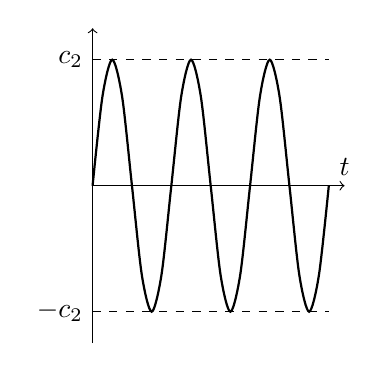
\begin{tikzpicture}[scale=2]
    \draw[->](0,0)--(1.6,0)node[above]{$t$};
    \draw[->](0,-1)--(0,1);
    \draw[dashed](0,0.8)node[left]{$c_2$}--(1.5,0.8);
    \draw[dashed](0,-0.8)node[left]{$-c_2$}--(1.5,-0.8);
    \draw[thick,smooth, domain=0:1.5]plot (\x,{0.8*sin(4*pi*\x r)});
\end{tikzpicture}
\end{document}